\section{Background}

\textbf{TODO:}
\begin{enumerate}
\item Refer Sutton and Barto - Reinforcement Learning: An Introduction on Reinforcement Learning
\item 
\end{enumerate}

In this section we discuss the subjects that are crucial to understanding the complexities and scope of our research. We begin by exploring the core principles of Financial Markets with an emphasis on the Forex Market. Next we conduct an analysis of Neural Networks and Reinforcement Learning highlighting how these approaches converge to develop solutions for Forex trading. Lastly we explore the intersection of these two branches of machine learning through an exploration of Deep Reinforcement Learning.

\subsection{Financial Markets and Trading}
Financial markets play an important role in the global economy by facilitating the flow of capital, ensuring liquidity and managing risks. They provide a platform for entities to trade assets, hedge financial risks and fund their operations. These markets serve different purposes, Table~\ref{Tables:FinancialMarkets} displays an overview of the main financial markets and their respective economic role.

\begin{table}[htb!]
\caption{Summary of Financial Markets and respective Economic Role\cite{brandimarte_introduction_2018}.}
\label{Tables:FinancialMarkets}
\centering
\footnotesize
\begin{tabularx}{\textwidth}{@{}lXl@{}}
\toprule
\textbf{Market} & \textbf{Economic Role} & \textbf{Asset Examples} \\
\midrule
Stock Market & Capital raising through company shares trading. & Stocks, Equities \\
\addlinespace
Bond Market & Debt financing by entities borrowing from investors. & Government and Corporate Bonds \\
\addlinespace
Commodities Market & Trading of essential raw materials and agricultural goods. & Oil, Gold, Wheat \\
\addlinespace
Forex Market & Currency exchange for international trade. & USD, EUR, JPY, GPB \\
\addlinespace
Derivatives Market & Trading contracts for hedging or speculation. & Futures, Options, Swaps \\
\addlinespace
Indices Market & Aggregating and tracking market or sector performance. & S\&P 500, NASDAQ \\
\addlinespace
Cryptocurrency Market & Exchanging digital currencies. & Bitcoin, Ethereum \\
\bottomrule
\end{tabularx}
\end{table}


Although each market has its function they are interconnected in a way that means activity in one market can impact others. This highlights their importance. The behavior of these markets is influenced by a range of participants including investors and major financial institutions whose actions can influence asset prices and market trends.

Regulatory bodies play a role in maintaining the integrity of these markets by enforcing policies that protect investors and contribute to prosperity. Technological advancements such as trading platforms and algorithmic strategies have made the markets more accessible and sophisticated. However they also bring challenges like increased volatility and regulatory uncertainty.

The Forex market stands out due to its size and liquidity. Making it particularly suited for applying machine learning techniques. This study focuses on exploring the application of methods within this market domain. It aims to understand the dynamics of the Forex market as assess the feasibility of utilizing machine learning, in financial strategies.

\subsubsection{Forex Market: Characteristics and Significance}
The Foreign Exchange market, or Forex market, is a marketplace where currencies are exchanged. It is the worlds most liquid market operating continuously across different time zones due to the involvement of banks and institutions worldwide. The major currency pairs like EUR/USD and GBP/USD play a role in this market as they are widely traded and offer insights into geopolitical trends.

Forex trading is influenced by factors such as data, political events, interest rates and the use of leverage. Leverage allows investors to control significant positions with minimal capital, which amplifies both potential profits and losses. The unique features of Forex, including its liquidity, diverse participants and sensitivity to events make it an attractive subject for advanced financial research and algorithmic strategies.

Given its complexities and volatile nature the importance of Forex in finance cannot be understated. This is especially true for machine learning and AI applications. In the following section we will delve into the aspects of Forex trading by focusing on currency pair mechanics and fundamental concepts that need to be understood before delving into more complex predictive models.

\subsubsection{Fundamental Concepts in Forex Trading}
Trading currency pairs involves buying one currency while simultaneously selling another. For instance when you buy the EUR/USD pair you are essentially purchasing Euros and selling US Dollars based on your prediction that the Euro will strengthen against the Dollar. In this research we will be focusing on major currency pairs: EUR/USD, USD/JPY, GBP/USD, AUD/USD, USD/CHF, NZD/USD and USD/CAD. These pairs involve recognized currencies and offer valuable insights into global economic trends. Deciding whether to buy or sell a pair relies on predicting the strength of one currency compared to another.

Forex trading thrives in a decentralized market that operates globally. This means there is no exchange where all transactions take place. Instead a network of market makers primarily composed of banks (known as the interbank market) and brokers facilitate trades. Interbank transactions involve trades with large volumes. They are usually dominated by institutions like multinational corporations and major hedge funds due to their transaction sizes. On the hand retail traders participate in Forex trading through brokers who have access to the interbank network. These brokers serve as intermediaries, facilitating trading for investors by connecting them to the larger currency exchange network. Both market-makers and brokers are always ready to buy or sell currencies at quoted prices. The way they operate is by providing two prices publicly: the bid price (the price at which they are willing to buy a currency) and the ask price (the price at which they are willing to sell it). The difference between these two prices, known as the spread serves as a commission for market-makers and brokers. The absence of a central trading venue might suggest a lack of regulation, however, the Forex market is self-regulated by competition among market-makers. This competitive environment ensures that pricing remains fair and spreads are kept tight, thus preserving market integrity and transparency for all participants.

To understand the Forex market it is important to understand how traders interpret market movements. Candlestick charts are a popular approach in this regard as they provide a view of price fluctuations. Each candlestick represents price movements during a time span, which can vary from minutes to years. Each individual price movement is known as a tick and occurs when buyers and sellers agree on a price leading to adjustments in bid and ask prices in the order book.

\begin{figure}[htb!]
\centering
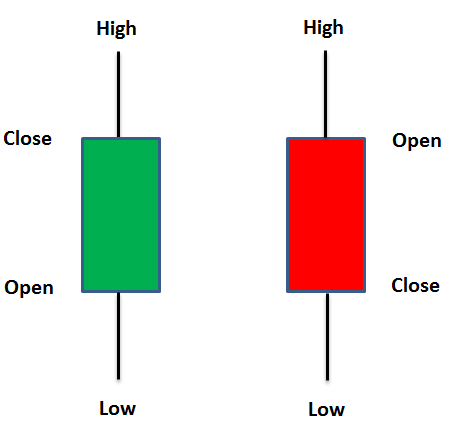
\includegraphics[width=0.3\textwidth]{Images/CandlestickChart.png}
\caption{Candlestick chart representation of upward and downward movements.}
\label{Figure:CandlestickChart}
\end{figure}

The structure of a candlestick (refer to Figure~\ref{Figure:CandlestickChart}) provides information about the opening (O), the highest (H), the lowest (L) and the closing (C) prices for a specific time period. The color of the candlestick represents the price movement with lighter shades indicating an increase and darker shades indicating a decrease. This allows traders to get an understanding of market direction. Although candlestick charts show price trends they do not directly display trading volume (V), a measure of the number of ticks or transactions. It is often shown on the chart as an additional indicator of market momentum.

This research relies on OHLCV data, which includes all the elements, for analyzing market behavior. It also incorporates indicators that interpret OHLCV data to help guide trading decisions following the analysis techniques used by traders.

\subsubsection{Predictive Analysis in Forex Trading}
Now we move from representing data in Forex trading to examining it for making informed trading decisions. Our main focus is on exploring methods that provide insights into the market and sustain predictive power. There are three main types of analysis:

\begin{itemize}
\item \textbf{Fundamental Analysis}: examines economic factors affecting currency prices. This includes analysis of GDP growth, employment rates, interest rates, and monetary policies, which help predict currency trends based on a nation's economic health. However, the qualitative nature of this data poses challenges for computational models that prefer structured numerical input.
\item \textbf{Sentiment Analysis}: seeks to quantify market mood by analyzing news, market commentary, and similar qualitative data. It aims to gauge how collective emotions impact market trends, although its complexity and need for advanced natural language processing make it less straightforward for model integration.
\item \textbf{Technical Analysis}: involves analyzing past price and volume data to predict future price movements. It operates on the principle that historical market behavior can forecast future trends.
\end{itemize}

The focus of this research will be on technical analysis, favored for its quantitative results that can be leveraged by complex machine learning models. There are four main types of technical indicators:

\begin{itemize}
\item \textbf{Trend Indicators}: Used to identify the prevailing direction of market by filtering out market noise. Refer to Table~\ref{Tables:TrendIndicators} for more details.
\item \textbf{Momentum Indicators}: Used to capture the momentum of a given trend, whether it is strong or weak and if a reversal is expected. Refer to Table~\ref{Tables:MomentumIndicators} for more details.
\item \textbf{Volume Indicators}: Used to provide a perspective on the trading volume, offering clues about the strength of a price movement. Refer to Table~\ref{Tables:VolumeIndicators} for more details.
\item \textbf{Volatility Indicators}: Used to identify the level of uncertainty or risk in the market associated with the volatility of the price movement. Refer to Table~\ref{Tables:VolatilityIndicators} for more details.
\end{itemize}

\begin{table}[htb!]
\caption{Summary of Trend Technical Indicators}
\label{Table:TrendIndicators}
\centering
\footnotesize
\begin{tabularx}{\textwidth}{@{}lXl@{}}
\toprule
\textbf{Indicator Name} & \textbf{Formula} & \textbf{Range} \\ 
\midrule
Simple Moving Average & $\text{SMA}(N)_t = \frac{1}{N} \sum_{i=1}^{N} \text{Price}_{t-N+i}$ & - \\
\addlinespace
Exponential Moving Average & $\text{EMA}(N)_t = \frac{2}{N+1} \times \text{Price}_t + (1 - \frac{2}{N+1}) \times \text{EMA}(N)_{t-1}$ & - \\
\addlinespace
Weighted Moving Average & $\text{WMA}(N)_t = \frac{2}{N \times (N + 1)} \sum_{i=1}^{N} i \times \text{Price}_{t-N+i}$ & - \\
\addlinespace
Double Exponential Moving Average & $\text{DEMA}(N)_t = 2 \times \text{EMA}(N)_t - \text{EMA}_2(N)_t$ & - \\
\addlinespace
Triple Exponential Moving Average & $\text{TEMA}(N)_t = 3 \times [\text{EMA}(N)_t - \text{EMA}_2(N)_t] + \text{EMA}_3(N)_t$ & - \\
\addlinespace
Hull Moving Average & $\text{HMA}(N)_t = \text{WMA}\left(2 \times \text{WMA}\left(\frac{N}{2}\right)_t - \text{WMA}(N)_t\right)$ & - \\
\addlinespace
Triangular Moving Average & $\text{TRIMA}(N)_t = \frac{1}{N} \sum_{i=1}^{N} \text{SMA}(N)_{t-N+i}$ & - \\
\addlinespace
Kaufman Adaptive Moving Average & $\text{KAMA}(N)_t = \text{KAMA}(N)_{t-1} + \text{SC} \times (\text{Price}_t - \text{KAMA}(N)_{t-1})$ & - \\
\addlinespace
& $\text{SC} = [ \text{ER} \times (\phi_{\text{short}} - \phi_{\text{long}}) + \phi_{\text{long}} ]^2, \phi_{\text{short}} = \frac{2}{N_{\text{short}} + 1}$, $\phi_{\text{long}} = \frac{2}{N_{\text{long}} + 1}$ & \\
\addlinespace
& $\text{ER} = \frac{| \text{Price}_t - \text{Price}_{t-N} |}{\sum_{i=1}^{N} | \text{Price}_{t-i+1} - \text{Price}_{t-i} |}$ & \\
\addlinespace
& where typically $N_{\text{short}} = 2$ and $N_{\text{long}} = 30$ & \\
\bottomrule
\end{tabularx}
\end{table}

\begin{table}[htb!]
\caption{Summary of Momentum Technical Indicators}
\label{Tables:MomentumIndicators}
\centering
\footnotesize
\begin{tabularx}{\textwidth}{@{}lXl@{}}
\toprule
\textbf{Indicator Name} & \textbf{Formula} & \textbf{Range} \\ 
\midrule
Price Momentum & $\text{PM}_t = \frac{\text{Price}_t - \text{Price}_{t-1}}{\text{Price}_{t-1}}$ & - \\
\addlinespace
Relative Strength Index & $\text{RSI}(N)_t = 100 - \frac{100}{1 + \frac{\text{Average Gain}_t}{\text{Average Loss}_t}}$ & [0, 100] \\
\addlinespace
& $\text{Average Gain}_t = \frac{1}{N}\sum_{i=1}^{N} \max(\text{Price}_i - \text{Price}_{i-1}, 0)$ & \\
\addlinespace
& $\text{Average Loss}_t = \frac{1}{N}\sum_{i=1}^{N} \max(\text{Price}_{i-1} - \text{Price}_i, 0)$ & \\
\addlinespace
Aroon Oscillator & $\text{Aroon}(N)_t = \text{Aroon Up}(N)_t - \text{Aroon Down}(N)_t$ & [-100, 100] \\
\addlinespace
& $\text{Aroon Up}(N)_t = \left( \frac{N - \text{Periods Since Highest High in } N}{N} \right) \times 100$ & \\
\addlinespace
& $\text{Aroon Down}(N)_t = \left( \frac{N - \text{Periods Since Lowest Low in } N}{N} \right) \times 100$ & \\
\addlinespace
Balance of Power & $\text{BOP}_t = \frac{\text{Close}_t - \text{Open}_t}{\text{High}_t - \text{Low}_t}$ & [-1, 1] \\
\addlinespace
Commodity Channel Index & $\text{CCI}(N)_t = \frac{\text{TP}_t - \text{SMA}_\text{TP}(N)_t}{0.015 \times \text{Mean Deviation}(N)_t}$ & - \\
\addlinespace
& $\text{TP}_t = \frac{\text{High}_t + \text{Low}_t + \text{Close}_t}{3}$ & \\
\addlinespace
& $\text{Mean Deviation}(N)_t = \frac{1}{N}\sum_{i=1}^{N} |\text{TP}_i - \text{SMA}_\text{TP}(N)_t|$ & \\
\addlinespace
Moving Average Convergence Divergence & $\text{MACD}_t = \text{EMA}(N_{\text{short}})_t - \text{EMA}(N_{\text{long}})_t $ & - \\
\addlinespace
& where typically $N_{\text{short}} = 12$ and $N_{\text{long}} = 26$ & \\
\addlinespace
Stochastic RSI & $\text{StochRSI}(N)_t = \frac{\text{RSI}(N)_t - \max(\text{RSI}(N))}{\max(\text{RSI}(N)) - \min(\text{RSI}(N))}$ & [0, 100] \\
\addlinespace
Stochastic Oscillator & $\text{Stoch \%K}(N)_t = \frac{\text{Close}_t - \text{LL}(N)_t}{\text{HH}(N)_t - \text{LL}(N)_t} \times 100$ & [0, 100] \\
\addlinespace
& $\text{Stoch \%D}(M)_t = \text{SMA}_{\text{Stoch \%K}(N)}(M)_t$ & [0, 100] \\
\addlinespace
& $\text{HH}(N)_t = \max_{i=t-N+1}^{t}(\text{High}_i)$, $\text{LL}(N)_t = \min_{i=t-N+1}^{t}(\text{Low}_i)$ & \\
\addlinespace
Ultimate Oscillator & $\text{UO}_t = \frac{4 \times \text{Avg}_t(N_1) + 2 \times \text{Avg}_t(N_2) + \text{Avg}_t(N_3)}{4+2+1} \times 100$ & [0, 100] \\
\addlinespace
& $\text{Avg}_t(N) = \frac{\sum_{i=0}^{N-1}\text{BP}_{t-i}}{\sum_{i=0}^{N-1}\text{TR}_{t-i}}$ & \\
\addlinespace
& $\text{BP}_t = \text{Close}_t - \min(\text{Close}_{t-1}, \text{Low}_t)$ & \\
\addlinespace
& $\text{TR}_t = \max(\text{Close}_{t-1}, \text{High}_t) - \min(\text{Close}_{t-1}, \text{Low}_t)$ & \\
\addlinespace
& where typically $N_1 = 7$, $N_2 = 14$, and $N_3 = 28$ & \\
\addlinespace
Williams \%R & $\text{Williams \%R}(N)_t = \frac{\text{HH}(N)_t - \text{Close}_t}{\text{HH}(N)_t - \text{LL}(N)_t} \times -100$ & [-100, 0] \\
\bottomrule
\end{tabularx}
\end{table}

\begin{table}[htb!]
\caption{Summary of Volume Technical Indicators}
\label{Tables:VolumeIndicators}
\centering
\footnotesize
\begin{tabularx}{\textwidth}{@{}lXl@{}}
\toprule
\textbf{Indicator Name} & \textbf{Formula} & \textbf{Range} \\ 
\midrule
Chaikin Accumulation/Distribution Line & $\text{AD}_t = \text{AD}_{t-1} + \text{MFV}_t$ & - \\
\addlinespace
& $\text{MFV}_t = \frac{\text{Close}_t - \text{Low}_t}{\text{High}_t - \text{Low}_t} \times \text{Volume}_t$ & \\
\addlinespace
Chaikin Accumulation/Distribution Oscillator & $\text{ADOSC}_t = \text{EMA}_\text{AD}(N_{\text{short}})_t - \text{EMA}_\text{AD}(N_{\text{long}})_t$ & - \\
\addlinespace
& where typically $N_{\text{short}} = 3$ and $N_{\text{long}} = 10$ & \\
\addlinespace
On-Balance Volume & $\text{OBV}_t = 
\begin{cases} 
\text{OBV}_{t-1} + \text{Volume}_t & \text{if } \text{Price}_t > \text{Price}_{t-1} \\
\text{OBV}_{t-1} - \text{Volume}_t & \text{if } \text{Price}_t < \text{Price}_{t-1} \\
\text{OBV}_{t-1} & \text{otherwise}
\end{cases}$ & - \\
\bottomrule
\end{tabularx}
\end{table}

\begin{table}[htb!]
\centering
\footnotesize
\begin{tabularx}{\textwidth}{@{}lXl@{}}
\toprule
\textbf{Indicator Name} & \textbf{Formula} & \textbf{Range} \\ 
\midrule
Standard Deviation & $\text{SD}(N)_t = \sqrt{\frac{1}{N-1} \sum_{i=1}^{N} (\text{Price}_i - \overline{\text{Price}})^2}$ & - \\
\addlinespace
Bollinger Bands & $\text{Upper BB}(N, k)_t = \text{SMA}(N)_t + k \times \text{SD}(N)_t$ & - \\
\addlinespace
& $\text{Lower BB}(N, k)_t = \text{SMA}(N)_t - k \times \text{SD}(N)_t$ & \\
\addlinespace
& where typically $ k = 2 $& \\
\addlinespace
Average True Range & $\text{ATR}(N)_t = \frac{1}{N} \sum_{i=1}^{N} \text{TRANGE}_i$ & - \\
\addlinespace
& $\text{TRANGE}_t = \max(\text{High}_t - \text{Low}_t, |\text{High}_t - \text{Close}_{t-1}|, |\text{Low}_t - \text{Close}_{t-1}|)$ & \\
\addlinespace
Normalised Average True Range & $\text{NATR}(N)_t = \frac{\text{ATR}(N)_t}{\text{Close}_t} \times 100$ & - \\
\addlinespace
Chaikin Volatility Index & $\text{CVI}(N)_t = \frac{1}{N} \sum_{i=1}^{N} (\text{High}_i - \text{Low}_i)$ & - \\
\bottomrule
\end{tabularx}
\caption{Summary of frequently used Volatility Technical Indicators \cite{jansen_machine_2020}.}
\label{Tables:VolatilityIndicators}
\end{table}


Technical indicators provide traders with tools for conducting market analysis and making informed decisions. They have been playing an important role in manual trading over the years and more recently have been serving as fundamental components in sophisticated machine learning models that enhance market analysis.

\subsubsection{Algorithmic and Quantitative Trading}
The financial markets have evolved significantly, increasingly influenced by technology, leading to the predominance of machines and algorithms in trading strategies. 

Algorithmic Trading uses computer programs to execute trades far quicker and in greater volumes than human traders. It efficiently analyzes data, interprets market conditions, and executes trades based on set criteria. Used in pre-trade analysis, signal generation, and trade execution, it's integral for large institutions and hedge funds to implement complex strategies rapidly and on a large scale.

Quantitative Trading, driven by quants (quantitative analysts), advances this with mathematical and statistical models to find trading opportunities. It involves applying these models to market data to identify patterns and correlations, utilizing historical data analysis, machine learning, and algorithms. This data-centric approach demands a strong grasp of finance and mathematics, focusing on systematic strategies over human judgment.

Both algorithmic and quantitative trading have transformed financial markets, enhancing efficiency and introducing new dynamics like high-frequency trading (HFT). This blend of finance and technology has reshaped trading, highlighting the importance of advanced machine learning models like neural networks for analyzing complex market data and reinforcement learning for developing intelligent trading strategies.

\subsection{Neural Networks}
In todays world, where we have an abundance of data and easy access to it, the power of machine learning has become a game changer in  many fields. At its core, machine learning relies on algorithms to identify patterns in data and to make decisions with minimal human intervention. Tom Mitchell, a leading figure in the field from Carnegie Mellon University, explains it as:
\begin{quote}
"A computer program is said to learn from experience E with respect to some task T and some performance measure P, if its performance on T, as measured by P, improves with experience E."
\end{quote}
This captures the essence of machine learning: creating models that automatically improve through experience. Neural networks, the topic of this section, is a class of machine learning models that operate within this framework by simulating the complex networks of the human brain.

\subsubsection{Fundamentals and History}
Neural Networks (NN), named for their resemblance to the human brain's structure, are algorithms designed for pattern recognition. In the human brain, a neuron receives signals through structures called dendrites, processes these signals in the nucleus and passes the resultant processed signal down its axon to the dendrites of adjacent neurons. Similarly, in a neural network, each node represents an artificial neuron that receives input, processes it through a mathematical function and passes the output to the subsequent layer of nodes. In both cases the strength and nature of the connections between neurons determine the network's behavior. Refer to Figure~\ref{Figure:HumanNeuronVsArtificialNeuron} for a visual representation of the concepts explained above.

\begin{figure}[htb!]
\centering
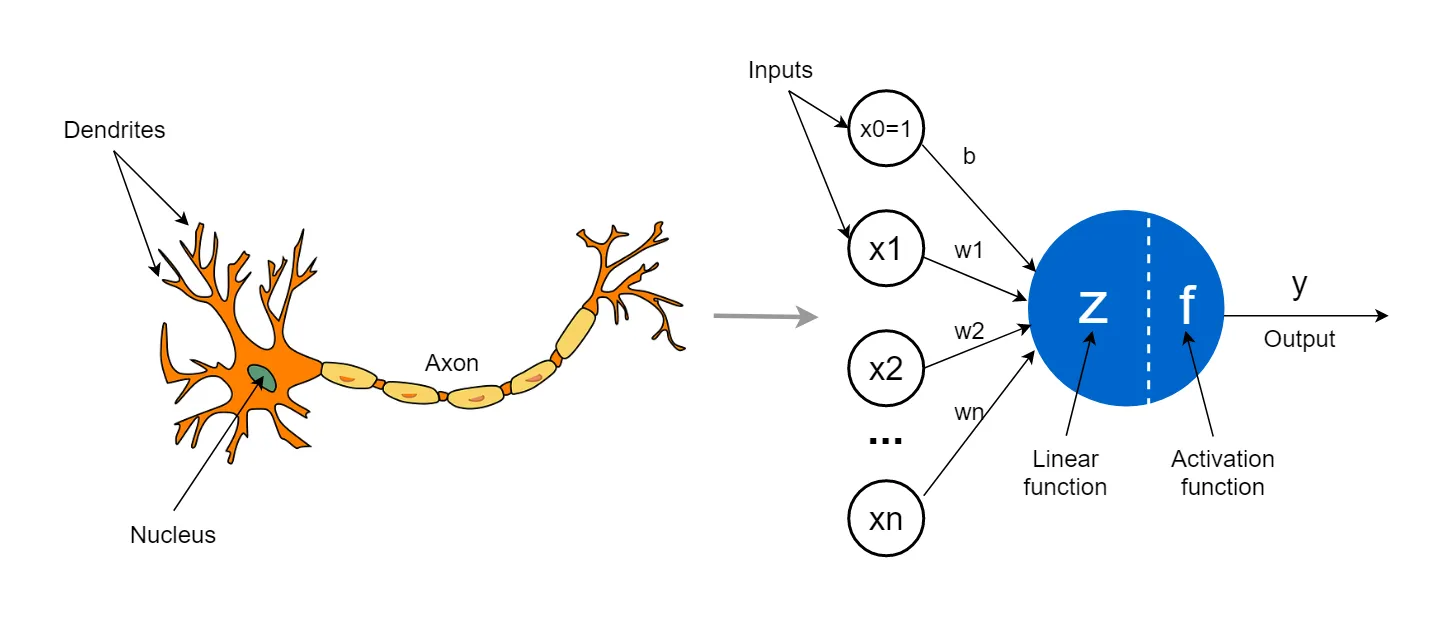
\includegraphics[width=0.7\textwidth]{Images/HumanNeuronVsArtificialNeuron.png}
\caption{Human Neuron compared to an Artificial Neuron.}
\label{Figure:HumanNeuronVsArtificialNeuron}
\end{figure}

The concept of neural networks dates back to the 1950s with the perceptron, a simple model of a biological neuron developed by Frank Rosenblatt. Initially limited to linearly separable datasets, the perceptron marked the early stages of neural network research. This field faced setbacks, leading to periods of reduced interest known as "AI winters." However, the 1980s brought a significant breakthrough with the backpropagation algorithm, enabling neural networks to learn from complex, multi-layered models.

\subsubsection{Technical Aspects and Feed-Forward}
In a neural network, the feed-forward computation within each layer \( l \) is predicated upon the data processed by its predecessor. For the first layer, this input \( x \) is the raw data itself, while for subsequent layers, it is the output from the previous layer \( h^{(l-1)}(x) \). The computation at each layer can be formalized as:

\begin{equation}
z^{(l)}(x) = W^{(l)} h^{(l-1)}(x) + b^{(l)}
\end{equation}

Here, the weight matrix \( W^{(l)} \in \mathbb{R}^{K_l \times K_{l-1}} \) and the bias vector \( b^{(l)} \in \mathbb{R}^{K_l} \) are required for the computation at layer \( l \), with \( K_l \) representing the number of neurons or units in layer \( l \), and \( K_{l-1} \) indicating the number of neurons in the preceding layer \( l-1 \). Specifically, \( W^{(1)} \in \mathbb{R}^{K_1 \times D} \) for the first layer, where \( D \) is the dimensionality of the input data. The activation function \( g \) is subsequently applied to the pre-activation \( z^{(l)}(x) \in \mathbb{R}^{K_l} \) to produce the activated output \( h^{(l)}(x) \in \mathbb{R}^{K_l} \):

\begin{equation}
h^{(l)}(x) = g(z^{(l)}(x))
\end{equation}

During the design of a neural network, the choice for the activation functions is very important. The choice of activation function for the hidden layers may employ a variety of non-linear activation functions, adding layers of expressiveness to the network that allow it to learn more complex patterns. On the other hand, the activation function utilized in the output layer is determined by the type of task the network is going to perform. It is this careful selection that directly influences the network's proficiency in accurately and effectively modeling the data. Refer to Table~\ref{Tables:ActivationFunctions} for a summarized overview of the main activation functions.

\begin{table}[htb!]
\caption{Summary of Important Activation Functions}
\label{Table:ActivationFunctions}
\centering
\footnotesize
\begin{tabularx}{\textwidth}{@{}lXl@{}}
\toprule
\textbf{Activation Function} & \textbf{Formula} & \textbf{Description} \\
\midrule
Linear & \( a(x) = x \) & Suitable for regression tasks. \\
\addlinespace
Sigmoid & \( \sigma(x) = \frac{1}{1 + e^{-x}} \) & Maps inputs to (0, 1), for binary classification. \\
\addlinespace
Hyperbolic Tangent & \( \tanh(x) = \frac{e^{x} - e^{-x}}{e^{x} + e^{-x}} \) & Maps inputs to (-1, 1), offering richer gradients than sigmoid. \\
\addlinespace
ReLU & \( \text{ReLU}(x) = \max(0, x) \) & Encourages sparse activation, helps with gradient flow. \\
\addlinespace
Softmax & \( \text{Softmax}(z)_i = \frac{e^{z_i}}{\sum_{k=1}^K e^{z_k}} \) & Turns logits into probabilities, for multi-class classification. \\
\bottomrule
\end{tabularx}
\end{table}


\subsubsection{Learning and Optimization using Backpropagation}
Neural networks learn by iteratively adjusting weights and biases to minimize the error between predicted outputs and actual target values. This learning process is guided by a loss function that quantifies the model's error. The goal is to optimize the network by finding parameters that minimize this loss function. Different problems require different loss functions, such as mean squared error for regression tasks and cross-entropy for classification. Refer to Table~\ref{Tables:LossFunctions} for a detailed overview of their formulas.

\begin{table}[htb!]
\centering
\footnotesize
\begin{tabularx}{\textwidth}{@{}lXl@{}}
\toprule
\textbf{Loss Function} & \textbf{Formula} & \textbf{Application} \\
\midrule
Mean Squared Error (MSE) & \( \frac{1}{n} \sum_{i=1}^n (y_i - \hat{y}_i)^2 \) & Regression \\
\addlinespace
Negative Log-Likelihood (Cross-Entropy) & \( -\sum_{i=1}^n y_i \log(\hat{y}_i) \) & Classification \\
\bottomrule
\end{tabularx}
\caption{Summary of the most common Loss Functions \cite{goodfellow_deep_2016}.}
\label{Tables:LossFunctions}
\end{table}


The core algorithm used to train neural networks is known as backpropagation. It involves calculating the gradients of the loss function relative to the network's weights and biases, which mathematically indicates the steepest increase in the loss function. Refer to Algorithm~\ref{Codes:GradientLossFunction} for a detailed overview of how to calculate these gradients.

\begin{algorithm}[htb!]
\caption{Gradient of the Loss Function}
\label{Codes:GradientLossFunction}
\begin{algorithmic}
\REQUIRE \( f \): network function, \( \theta \): network parameters, \( x \): input data, \( y \): true label, \( l \): number of layers, \( L \): loss function
\STATE Compute the output of the network \( \hat{y} = f(x; \theta) \)
\STATE Compute the gradient of the loss function with respect to the output layer before activation:
\STATE \( \nabla_{z^{(l+1)}}L(f(x; \theta), y) = \frac{\partial L(f(x; \theta), y)}{\partial \hat{y}} \cdot \frac{\partial \hat{y}}{\partial z^{(l+1)}} \)
\FOR{\( \ell = l+1 \) to \( 1 \)}
\STATE Compute gradients of hidden layer parameters:
\STATE \( \nabla_{W^{(\ell)}}L(f(x; \theta), y) = \nabla_{z^{(\ell)}}L(f(x; \theta), y) \cdot h^{(\ell-1)T} \)
\STATE \( \nabla_{b^{(\ell)}}L(f(x; \theta), y) = \nabla_{z^{(\ell)}}L(f(x; \theta), y) \)
\STATE Compute gradient of previous hidden layer:
\STATE \( \nabla_{h^{(\ell-1)}}L(f(x; \theta), y) = W^{(\ell)T} \cdot \nabla_{z^{(\ell)}}L(f(x; \theta), y) \)
\STATE Compute gradient of previous hidden layer (before activation):
\STATE \( \nabla_{z^{(\ell-1)}}L(f(x; \theta), y) = \nabla_{h^{(\ell-1)}}L(f(x; \theta), y) \odot g'(z^{(\ell-1)}) \)
\ENDFOR
\end{algorithmic}
\end{algorithm}


Then, gradient descent algorithm is used to iteratively update the weights and biases in the opposite direction of the gradients, thus reducing the loss and hopefully increasing the network's accuracy. Its variants, outlined with respective formulas in Table~\ref{Tables:GradientDescent}, address different data and computational needs. Batch gradient descent uses the entire dataset for updates, ensuring thoroughness but potentially struggling with large datasets. Stochastic gradient descent updates parameters per data point, offering speed at the cost of stability. Mini-batch gradient descent strikes a balance, using data subsets for more stable and computationally efficient updates.

\begin{table}[htb!]
\caption{Summary of Gradient Descent Variants}
\label{Tables:GradientDescent}
\centering
\footnotesize
\begin{tabularx}{\textwidth}{@{}lXl@{}}
\toprule
\textbf{Algorithm} & \textbf{Formula} & \textbf{Description} \\
\midrule
Batch Gradient Descent & \(\theta := \theta - \eta \cdot \nabla_{\theta} J(\theta; X, y)\) & Updates parameters using all data \\
\addlinespace
Mini-Batch Gradient Descent & \(\theta := \theta - \eta \cdot \nabla_{\theta} J(\theta; X^{(i:i+n)}, y^{(i:i+n)})\) & Updates parameters using subsets of data \\
\addlinespace
Stochastic Gradient Descent & \(\theta := \theta - \eta \cdot \nabla_{\theta} J(\theta; x^{(i)}, y^{(i)})\) & Updates parameters per data point \\
\bottomrule
\end{tabularx}
\end{table}


In Table~\ref{Tables:GradientDescent}, the learning rate \( \eta \) is an hyperparameter that influences the convergence of gradient descent. An optimal learning rate balances convergence speed and precision, preventing overshooting or slow progress that could get trapped in local minima. Adaptive learning rate techniques, adjusting \( \eta \) during training, enhance learning efficacy, emphasizing the balance between convergence speed and accuracy in neural network training. Some other techniques to enhance convergence and its speed involve normalization and standardization of the input data.

\subsubsection{Bias-Variance Trade-off and Model Generalization}
The generalization power of a neural network, depends on finding balance between bias and variance. Bias leads to underfitting, where the model overlooks underlying trends due to overly simplistic assumptions, while variance leads to overfitting, where the model interprets noise as signal due to excessive complexity.

Both underfitting and overfitting result in bad performance of the model on new data, a significant issue in forex trading, where accurate market signal detection is essential. Cross-validation is employed to evaluate a model's generalization power to independent datasets. Additionally, regularization techniques like L1 and L2 regularization are used to moderate model complexity by adding penalties to the loss function. Dimensionality reduction can further help finding the right balance between bias and variance.

Implementing these strategies increase the change of training a model with more generalization power thus being able to perform in out-of-sample data. While important, these techniques are not the primary focus of this research and will not be explored in full detail.

\subsubsection{Universal Approximation Theorem}
The Universal Approximation Theorem, firstly introduced by George Cybenko in 1989 and later extended by Kurt Hornik in 1991, attributes a crucial characteristic to neural networks. It states that:

\begin{quote}
"A Neural Network with one hidden layer and a linear output can approximate arbitrarily well any continuous function, given enough hidden units."
\end{quote}

This theorem validates the capacity of neural networks to serve as universal function approximators. Another important result is from Montufar et al. (2014). It states that:
\begin{quote}
"The number of linear regions carved out by a deep neural network with D inputs, depth L, and K hidden units per layer with ReLU activations is \(O\left(\left(\frac{K}{D}\right)^{D(L-1)}K^D\right)\)."
\end{quote}

This means that, for fixed number of hidden units, deeper networks are exponentially more expressive. This results are important in the context of creating predictive models for forex trading using neural networks because, in theory, they should capture the underlying complex patterns that drive market movements.

\subsection{Reinforcement Learning}
Reinforcement Learning (RL) is a type of machine learning that focuses on an agents ability to interact with its environment and make decisions. Unlike other types of learning methods, RL emphasizes decision making on possibly complex and uncertain environments. The goal of RL is to maximize long term rewards by learning from the consequences of actions, through trial and error. This approach has found applications in a range of fields such, as robotics and finance enabling the development of systems that improve their performance over time adapt to new situations and make a series of decisions to achieve desired outcomes.

\subsubsection{Fundamentals and History}
The fundamentals of Reinforcement Learning are deeply rooted, in the principles of behaviorist psychology and optimal control theory within the context of Markov Decision Processes (MDPs). The history of RL can be traced back to the exploration of trial and error learning mechanisms in the 1950s. In the 1960s MDPs were formalized, providing a framework for modeling decision making situations. However it wasn't until the 1980s when computational power and algorithms became more advanced that RL started to gain momentum as a field. This era saw the introduction of concepts like Temporal Difference Learning and Q-Learning.

During this time various disciplines such as psychology, neuroscience, computer science and operations research came together, contributing to the growth of RL. The influential work of Richard S. Sutton and Andrew G. Barto in their book "Reinforcement Learning; An Introduction" was crucial in bringing cohesion to this field.
Their research established the core algorithms and theoretical foundations of Reinforcement Learning (RL) which paved the way for a surge in interest during the following century. RL proved to be effective in solving complex problems like game playing, autonomous navigation and financial market trading.

\subsubsection{Key Concepts and Theoretical Foundations}
Reinforcement Learning is about how an agent interacts with its environment. This interaction involves states, actions and rewards. The state \( S_t \) represents the situation of the agent. When the agent observes \( S_t \) it chooses an action \( A_t \). This action causes the environment to transition to a state \( S_{t+1} \), providing feedback in the form of a reward \( R_{t+1} \). Refer to Figure \ref{Figure:AgentEnvironment} for a visual representation of this cyclical interaction. 

\begin{figure}[htb!]
\centering
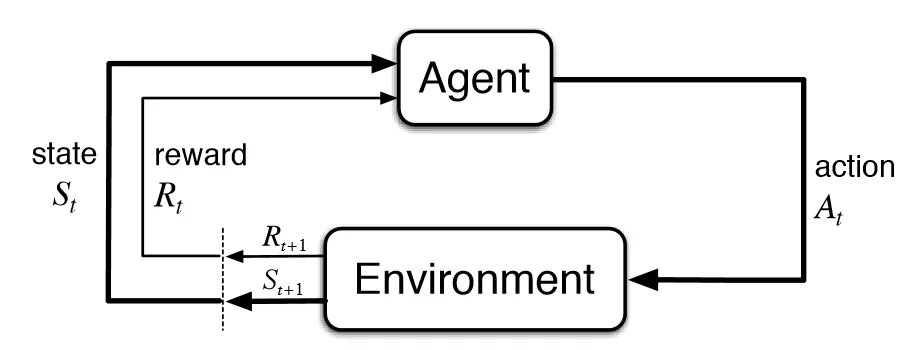
\includegraphics[width=0.6\textwidth]{Images/AgentEnvironment.png}
\caption{Interaction between the agent and the environment in a Reinforcement Learning setting.}
\label{Figure:AgentEnvironment}
\end{figure}

The main objective of the agent is to maximize its sum of rewards also known as the return. The return is basically the expected gain that can be achieved starting from state \( S_t \) as expressed by this formula:

\begin{equation}
R_{t+1} + \gamma R_{t+2} + \gamma^2 R_{t+3} + \ldots = \sum_{k=0}^{\infty} \gamma^k R_{t+k+1}
\end{equation}

Here, \( \gamma \) represents the discount factor, indicating the degree to which future rewards are considered relative to immediate ones. A policy \( \pi \) directs the agent's actions, which can be deterministic, assigning a specific action to each state, or stochastic, assigning a probability distribution over actions. Balancing exploration—the act of trying new actions to discover their effects—and exploitation—the act of choosing actions that are known to yield high rewards—is a fundamental challenge in RL. An important approach to this problem is the \(\varepsilon\)-greedy policy, which predominantly exploits the best-known action but occasionally explores random actions, thus ensuring both robustness and continual learning.

The fundamental concept, behind Reinforcement Learning (RL) lies in the Markov Decision Process (MDP) which can be defined using the tuple \( (S, A, P, R, \gamma) \). MDPs rely on the Markov property, which states that the likelihood of transitioning to the state is determined solely by the state and action taken without considering any past states or actions. Mathematically speaking;

\begin{equation}
\label{Equation:MarkovProperty}
P(s_{t+1} | s_t, a_t, s_{t-1}, a_{t-1}, \ldots, s_0, a_0) = P(s_{t+1} | s_t, a_t)
\end{equation}

The reward function is very important as it captures the agents objectives. It offers a signal that directs the agent towards achieving the goals of a task but it does not prescribe how to accomplish them. For example, in trading context, rewards can mirror gains and losses guiding the agent to adopt strategies that maximize profits.

\subsubsection{Value Functions and Q-Functions}
The value function for a policy \( \pi \), denoted as \( V^\pi(s) \), represents the expected return when starting in state \( s \) and following policy \( \pi \) afterwards. It is formulated as:

\begin{equation}
V^\pi(s) = \mathbb{E} \left[ \sum_{k=0}^{\infty} \gamma^k R_{t+k+1} \mid S_t = s, \pi \right]
\end{equation}

The Q-function for a policy \( \pi \), denoted as \( Q^\pi(s, a) \), represents the expected return for taking an action \( a \) in state \( s \) and following policy \( \pi \) afterwards. It is formulated as:

\begin{equation}
Q^\pi(s, a) = \mathbb{E} \left[ \sum_{k=0}^{\infty} \gamma^k R_{t+k+1} \mid S_t = s, A_t = a, \pi \right]
\end{equation}

The Bellman equations, named after Richard Bellman who first formulated them, provide a recursive decomposition for the total cumulative reward an agent can expect to receive starting from a particular state or state-action pair. These equations are fundamental to dynamic programming techniques in RL, as they express the relationship between the value of the current state or action and the expected values of subsequent states or actions. Following Bellman equation it is possible to obtain:

\begin{equation}
V^\pi(s) = \sum_{a \in A} \pi(a|s) \sum_{s' \in S} P(s'|s,a) \left[ R(s,a,s') + \gamma V^\pi(s') \right]
\end{equation}

\begin{equation}
Q^\pi(s, a) = \sum_{s' \in S} P(s'|s,a) \left[ R(s,a,s') + \gamma \sum_{a' \in A} \pi(a'|s') Q^\pi(s', a') \right]
\end{equation}

\begin{equation}
\label{Equation:RelationshipValueQFunction}
V^\pi(s) = \sum_{a \in A} \pi(a|s) Q^\pi(s, a)
\end{equation}

The relationship pointed in Equation~\ref{Equation:RelationshipValueQFunction} indicates that the value of a state under policy \( \pi \) is the expected value of the Q-function over all possible actions, weighted by the policy's action probabilities.

For optimal policies, we define the optimal value function \( V^*(s) \) and the optimal Q-function \( Q^*(s, a) \), which represent the maximum possible returns achievable from any state or state-action pair, respectively. Following Bellman equation it is possible to obtain:

\begin{equation}
V^*(s) = \max_{a \in A} \sum_{s' \in S} P(s'|s,a) \left[ R(s,a,s') + \gamma V^*(s') \right]
\end{equation}
\begin{equation}
Q^*(s, a) = \sum_{s' \in S} P(s'|s,a) \left[ R(s,a,s') + \gamma \max_{a' \in A} Q^*(s', a') \right]
\end{equation}
\begin{equation}
V^*(s) = \max_{a \in A} Q^*(s, a)
\end{equation}

Through iterative application of these equations, RL algorithms gradually approximate the value and Q-functions, guiding the agent towards the optimal policy that maximizes the expected cumulative reward.

\subsubsection{Methodological Variants and Learning Methods}
The field of reinforcement learning can be divided into categories based on the properties of learning: model-based versus model-free, on-policy versus off-policy strategies and value-based versus policy-based techniques.

In model-based RL, algorithms create a model of the environment to simulate and predict the outcomes of actions. This allows the agent to plan by forecasting states. This is possible when the environment is simple enough to be modeled. On the other hand, in model-free RL, algorithms directly learn a policy or value function from their interactions with the environment without explicitly modeling it. Model-free approaches are often chosen for environments where modeling is challenging or when an accurate model is not available.

Within the realm of model-free RL, there are on-policy strategies, which learn about the policy that is currently used to make decisions, and off-policy strategies, which explore a different policy while aiming to learn an optimal one.

Another important distinction lies between value-based and policy-based learning approaches. On the one hand, value-based methods, like Temporal Difference Learning (TD), Q-Learning and SARSA Learning, focus on estimating the value of states or state-action pairs. These algorithms derive policies implicitly from these values. SARSA Learning uses an on-policy strategy while Q-Learning and TD Learning use an off-policy strategy. On the other hand, policy-based methods, such as the REINFORCE Learning directly optimize the policy itself. These techniques are particularly useful when dealing with dimensional or continuous action spaces. 

In particular, Actor-Critic Learning combines elements of both policy-based and value-based approaches. It has a policy function (the actor) and a value function (the critic) which provides the stability and efficiency of value based-methods along with direct policy improvement. This collaboration between the actor and the critic result in improved policy updates, especially beneficial for complex environments. This algorithm is of particular relevance because it acts as a connection between reinforcement learning and neural networks, as we will see in the next section. Refer to Algorithm~\ref{Codes:ActorCritic} for a detailed implementation.

\begin{algorithm}[htb!]
\caption{Actor-Critic}
\label{Codes:ActorCritic}
\begin{algorithmic}
\REQUIRE $\pi(s, a; \theta)$: a differentiable policy, $Q(s, a; w)$: a differentiable $Q$-function, $N$: number of iterations and learning rates $\beta^\theta > 0$ and $\beta^w > 0$
\STATE Initialize policy parameter $\theta^{(0)}$ and $Q$-function parameter $w^{(0)}$
\STATE Initialize state $s$
\FOR{$n = 0, 1, \ldots, N - 1$}
    \STATE Sample $a \sim \pi(s, a; \theta^{(n)})$
    \STATE Take action $a$, observe state $s'$ and reward $r$
    \STATE Sample action $a' \sim \pi(s', a; \theta^{(n)})$
    \STATE Compute the TD error: $\delta \gets r + \gamma Q(s', a'; w^{(n)}) - Q(s, a; w^{(n)})$
    \STATE Update $w$: $w^{(n+1)} \gets w^{(n)} + \beta^w \delta \nabla_w Q(s, a; w^{(n)})$
    \STATE Update $\theta$: $\theta^{(n+1)} \gets \theta^{(n)} + \beta^\theta \delta \nabla_\theta \ln \pi(s, a; \theta^{(n)})$
    \STATE $s \gets s'$, $a \gets a'$
\ENDFOR
\end{algorithmic}
\end{algorithm}


While the Puterman theorem guarantees a deterministic stationary optimal policy for Markov Decision Processes (MDPs), such assurances do not extend to complex, non-stationary environments like financial markets. Forex markets, in particular, are influenced by historical data in ways that standard state representations in MDPs do not account for. Consequently, RL in these markets relies on approximated models, utilizing technical indicators and feature engineering to integrate essential historical information into the state representation in order to try to approximate the Markov property.

\subsection{Deep Reinforcement Learning}
Deep Reinforcement Learning (DRL) merges reinforcement learning's decision-making with the pattern recognition capabilities of neural networks, making it especially powerful for handling complex, high-dimensional data in environments like the forex market. DRL empowers trading algorithms with adaptability, positioning them to potentially revolutionize trading strategies.

\subsubsection{Fundamentals and History}
The rise of DRL as a new field within machine learning gained momentum when it became clear that neural networks could greatly enhance the capabilities of reinforcement learning agents in dealing with and understanding complex environments.

DeepMinds groundbreaking work, which demonstrated the success of the Deep Q Network (DQN) algorithm in mastering a range of Atari 2600 games using inputs marked a significant breakthrough for DRL. This achievement not only validated the efficacy of DRL in mastering high-dimensional state spaces but also highlighted its potential applicability to financial markets. In this context the challenge lies not in interpreting amounts of data but also in extracting strategic insights that can guide real time trading decisions. This historical advance, along with ongoing research, has sparked interest in applying DRL to forex trading. The field's evolution reflects a broader ambition: to harness the intricacy of market signals and evolve strategies that are resilient and dynamic.

\subsubsection{Deep Value-Based RL Algorithms: Deep Q-Networks}
Deep learning has transformed traditional value-based reinforcement learning methods, giving rise to what is known today as deep value-based methods. These advanced algorithms employ neural networks, renowned for their function approximation capabilities, to manage and interpret larger state spaces. Such an approach enables agents to learn and operate effectively in environments with complex, high-dimensional sensory input, a task that conventional value-based methods could not scale to efficiently.

Neural Fitted Q-Learning was one of the early techniques that laid the foundation for deep value-based learning. It utilizes neural networks to approximate the Q-function, which represents the expected return of a given state-action pair. By fitting a neural network to the Q-values obtained from completed episodes, it significantly enhanced the agent's ability to generalize across states in large and continuous spaces.

Nevertheless, the field of deep value-based methods truly came into prominence with the introduction of the Deep Q-Network (DQN) algorithm by Mnih et al. DQN integrated key innovations such as a separate target network for stabilizing the learning targets and an experience replay mechanism for breaking the temporal correlations within training batches. This approach allowed DQN to effectively learn control policies directly from high-dimensional inputs, a significant leap forward in the application of RL.

Following DQN, improvements such as the Double Deep Q-Network (DDQN) have been made to address limitations in the DQN architecture. DDQN mitigates the overestimation bias of action values by decoupling the action selection from the action evaluation. This is achieved by employing two networks: a primary network for action selection and a target network for evaluation, enhancing the stability and accuracy of the value estimation process.

Although deep value based methods are foundational and revolutionary, they will not be the focus of this research.

\subsubsection{Deep Policy-Based RL Algorithms: Deep Deterministic Policy Gradient}
Deep policy-based RL algorithms excel in environments with continuous action spaces. Unlike value-based methods that assign a value to each potential action, policy-based approaches directly optimize the policy to maximize expected returns. This quality is invaluable in the domain of forex trading, characterized by a vast and continuous action space that demands both precision and adaptability.

Among these approaches, the Deep Deterministic Policy Gradient (DDPG) algorithm stands out as a model-free off-policy actor-critic algorithm specifically designed for continuous action spaces. By combining the direct policy optimization of policy-based methods with the evaluation power of value-based approaches, DDPG achieves a stable and robust learning process. The algorithm consists of an actor component for selecting actions and a critic component that evaluates the actions by estimating their Q-values.

\begin{algorithm}[htb!]
\caption{Deep Deterministic Policy Gradient}
\label{Code:DeepDeterministicPolicyGradient}
\begin{algorithmic}
\REQUIRE an actor $\pi(s; \theta)$, a critic network $Q(s, a; \phi)$, learning rates $\beta$ and $\hat{\beta}$, initial parameters $\theta^{(0)}$ and $\phi^{(0)}$
\STATE Initialize target network parameters $\hat{\phi} \leftarrow \phi^{(0)}$ and $\hat{\theta} \leftarrow \theta^{(0)}$, replay buffer $\mathcal{B}$
\FOR{episode $= 1, M$}
    \STATE Initialize a random process $\mathcal{N}$ for action exploration
    \STATE Receive initial observation state $s_1$
    \FOR{t $= 1, T$}
        \STATE Select action $a_t = \pi(s_t; \theta) + \mathcal{N}_t$ according to the current policy and exploration noise
        \STATE Execute action $a_t$ and observe reward $r_t$ and new state $s_{t+1}$
        \STATE Store transition $(s_t, a_t, r_t, s_{t+1})$ in $\mathcal{B}$
        \STATE Sample a random minibatch of $N$ transitions $(s_i, a_i, r_i, s_{i+1})$ from $\mathcal{B}$
        \STATE Set $y_i = r_i + \gamma Q'(s_{i+1}, \pi'(s_{i+1}; \hat{\theta}); \hat{\phi})$
        \STATE Update critic by minimizing the loss: $L = \frac{1}{N}\sum_i(y_i - Q(s_i, a_i; \phi))^2$
        \STATE Update the actor policy using the sampled policy gradient:
        \STATE $\nabla_{\theta} J \approx \frac{1}{N}\sum_i \nabla_a Q(s, a; \phi)|_{s=s_i, a=\pi(s_i)} \nabla_{\theta}\pi(s; \theta)|_{s_i}$
        \STATE Update the target networks:
        \STATE $\hat{\phi} \leftarrow \tau \phi + (1 - \tau) \hat{\phi}$
        \STATE $\hat{\theta} \leftarrow \tau \theta + (1 - \tau) \hat{\theta}$
    \ENDFOR
\ENDFOR
\end{algorithmic}
\end{algorithm}


In Algorithm~\ref{Codes:DeepDeterministicPolicyGradient} it can observed how DDPG utilizes neural networks to approximate both the actor and critic functions. This enables handling complex input dimensions commonly encountered in forex markets. The utilization of a replay buffer for experience storage and the strategic sampling of mini-batches are key features that enhance learning stability by mitigating the correlation between sequential data points. Furthermore, DDPG incorporates target networks, which are gradually updated versions of the actor and critic, to solidify the learning targets and encourages gradual improvement.

While we can not guarantee convergence of DDPG due to the partially observable nature of forex markets, its design for continuous policy adaptation presents a compelling approach to developing sophisticated trading strategies. The adaptability of DDPG to the evolving conditions of financial markets highlights its potential as a breakthrough in algorithmic trading.
